\section{Introduction}
\label{sec:introduction}

Future service organizations allocate work among humans, AI systems, and human--AI teams. Each choice changes expected service, cost, capacity, accountability, review burden, and exposure to correlated AI failures. Human--AI staffing is therefore an economic resource-allocation problem with hard operational and institutional constraints, not merely a scheduling toy. Research on human--AI interaction calls for explicit authority and oversight boundaries~\citep{amershi2019humanai,seeber2020machines}; service operations supplies capacity and reliability models~\citep{gans2003callcenters}; and sociotechnical analysis cautions that efficiency or a compact fairness proxy cannot stand in for stakeholder welfare~\citep{selbst2019fairness}.

Quantum optimization introduces a second adoption decision. Even if a statevector experiment concentrates probability on good candidates, using the quantum component may be irrational once classical alternatives, validation, delay, review, and risk costs are counted. Small noiseless demonstrations also do not establish QPU performance, wall-clock advantage, or scaling~\citep{preskill2018nisq,cerezo2021variational,bharti2022nisq}. Rigorous optimization benchmarks consequently emphasize standardized instances, strong counterfactuals, solution quality, resources, and reproducibility~\citep{koch2026qoblib}; application-centric frameworks additionally ask whether the complete workflow improves a meaningful task~\citep{finzgar2022quark}.

Q-OPS moves the question one level upward: \emph{when is there enough evidence to invoke quantum computation at all?} The architecture in \cref{fig:architecture} treats quantum computation as an optional expert after a strong classical stage and before an independent certificate and fallback. It distinguishes system-level benchmarking (a fixed stack), algorithm-level benchmarking (controlled solver comparison), and application-level benchmarking (incremental decision value for the same organizational problem). The frozen study reaches the second level only on selectively retained cores inside an application-oriented architecture.

\begin{figure*}[t]
\centering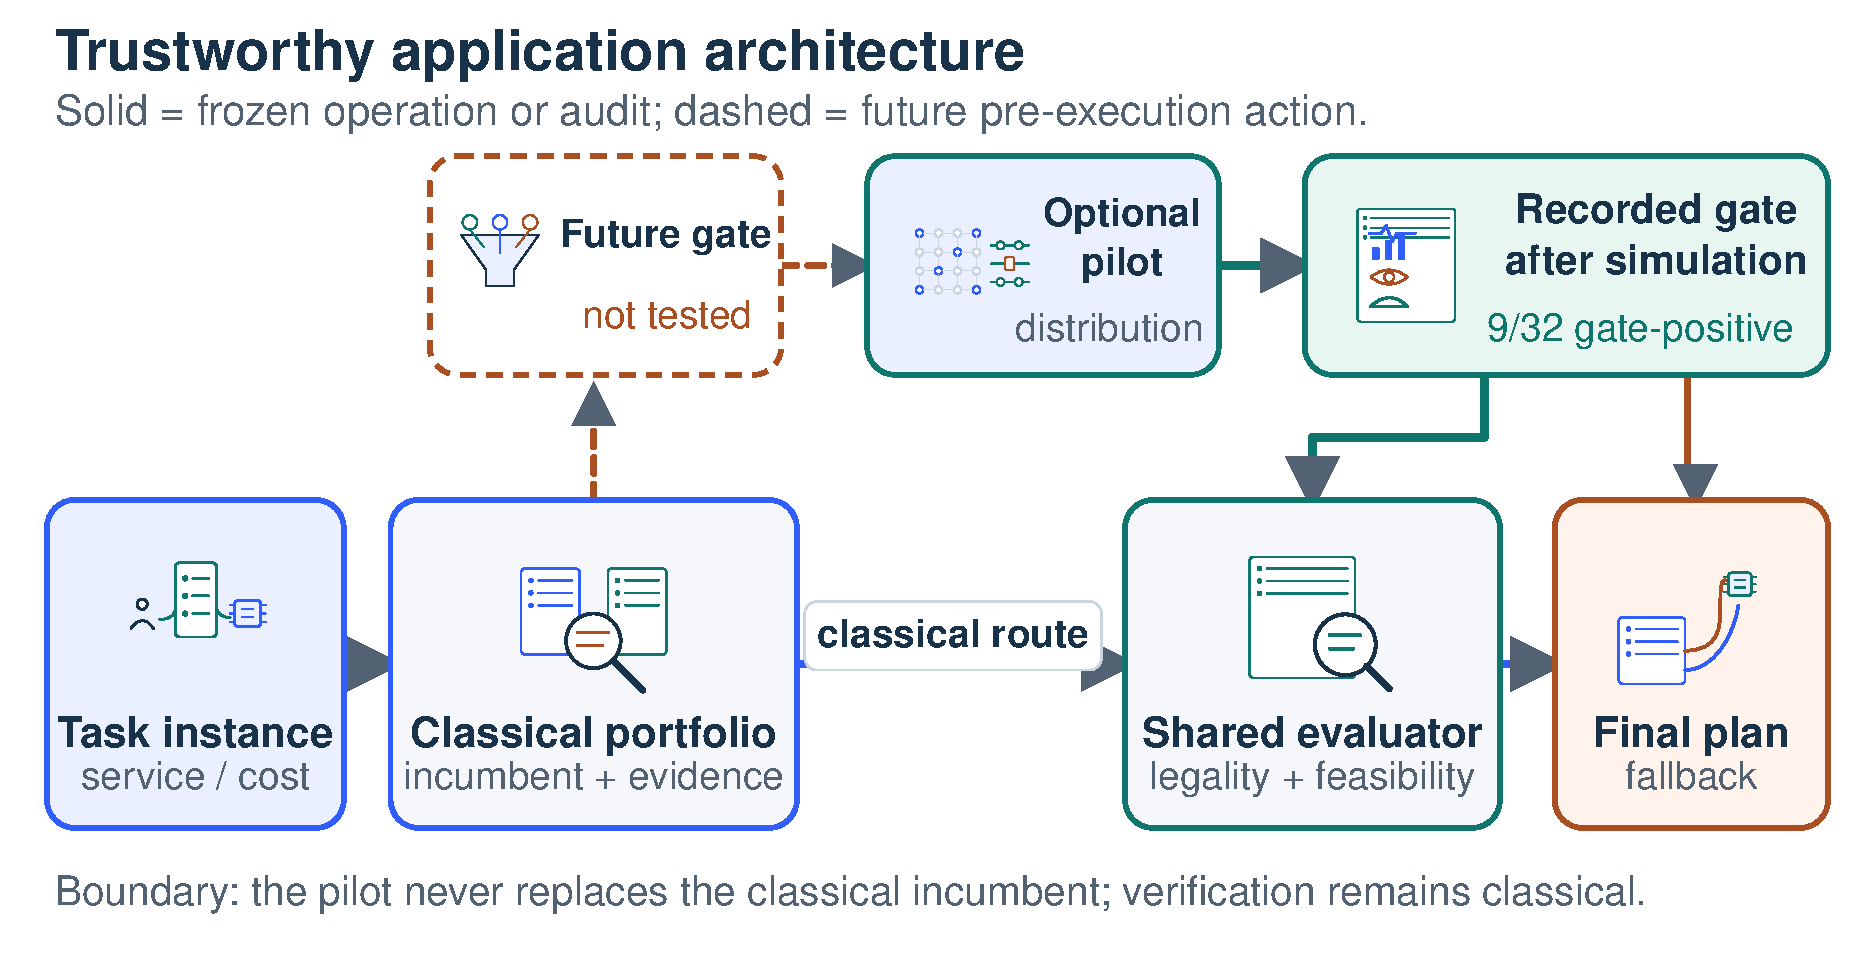
\includegraphics[width=\textwidth]{figs/fig1_architecture.pdf}
\caption{\textbf{Trustworthy application-level architecture.} Strong classical alternatives precede the recorded evidence gate; the quantum branch is optional; a shared classical evaluator and fallback bound operational acceptance. Dashed abstention/review is conceptual and was not evaluated. Clip art is semantic only; labels, arrows, gates, and evidence states are editable vector layers.}\label{fig:architecture}
\end{figure*}


The paper is organized around exactly three research-question--contribution pairs:
\begin{enumerate}[leftmargin=*,label=\textbf{RQ\arabic*.},itemsep=1pt,topsep=3pt]
\item \textbf{How can Human--AI staffing jointly represent service, cost, review scarcity, collaboration, correlated failures, and hard requirements?} We contribute a synthetic, governance-constrained benchmark with human-only, AI-only, and collaborative modes, empirical chance constraints, disruption scenarios, and an explicit composite feasibility predicate.
\item \textbf{When should a trustworthy decision system remain classical or run a quantum pilot?} We contribute an evidence-aware routing architecture driven by a multidimensional instance state, remaining classical headroom, ambiguity, feasibility, certification, and fallback. Abstention and human review are architectural actions, not evaluated policies in the frozen experiment.
\item \textbf{What conditional value survives strong counterfactuals and application-aware evidence boundaries?} We contribute a frozen, null-inclusive evaluation with matched sampling budgets, negative development stages, exact shared-field reproduction, and an evidence ladder that separates sampling improvement from optimization, application, and welfare claims.
\end{enumerate}

The headline result is deliberately two-sided. Nine of 32 held-out instances (28.13\%) satisfy the recorded post-simulation gate; across all 32 retained-core comparisons, $p=2$ statevector sampling has a 6.831$\times$ ratio of mean optimum probability over uniform feasible sampling. Independent evaluation records zero disallowed-mode violations, but composite feasibility holds for only 27/32 classical incumbents. The gate uses an observed quantum statistic and is not a prospective cost-saving router; $p=1$ exceeds $p=2$ on 28/32 cases under unequal search budgets; and stronger full-problem classical or hardware comparisons remain absent. A trustworthy system should maximize \emph{justified}, not maximal, quantum use.
